\documentclass[14pt,t,hyperref={colorlinks=true,urlcolor=red}]{beamer}

% Don't copy this template. It is pretty hacked up.
% Changes to make: 
%   - Make an environment for the standalone text to reduce the 
%     \center and \vspace commands

\usetheme{Rochester}                    % No navigation - simple theme

\usepackage{times}                      
\usefonttheme{structurebold}            % make titles bolder
\useinnertheme[shadow]{rounded}

\usepackage[english]{babel}             % not necessary?
\usepackage{pgf}                        % graphics
\usepackage[latin1]{inputenc}

\usepackage[urldate=iso8601,date=iso8601,style=numeric,defernumbers=true,backend=biber]{biblatex}


%\setbeamercovered{dynamic}              % no idea

% --------- SPOOKY FONT -------------------
\newcommand{\spooky}[1]{{\Huge \fontfamily{lgfz}\fontseries{m}\fontshape{n} \selectfont #1}}

% Use this if you do not have the Green Fuz font installed
% (But it is not spooky)
% 
% \newcommand{\spooky}[1]{{\Huge \textsc{#1}}}

% -------- ADDITIONAL PACKAGES -------------
\usepackage{orangeblack}
\usepackage{mdwlist}
\usepackage{fancyvrb}
\usepackage[T1]{fontenc}
\usepackage[scaled]{beramono}
\usepackage[normalem]{ulem}		% Strikeout effect

\setbeamercolor*{bibliography item}{fg=black}
\setbeamercolor*{bibliography entry title}{fg=black}
\setbeamercolor*{bibliography entry author}{fg=black}
\setbeamercolor*{bibliography entry location}{fg=black}
\setbeamercolor*{bibliography entry note}{fg=black}

% -------- LOCAL COMMANDS ------------

\newcommand{\code}[1]{{\usebeamercolor[fg]{structure}\texttt{#1}}}
\newcommand{\highlight}[1]{{\usebeamercolor[theme-bg]{structure}{#1}}}
\newcommand{\hl}[1]{{\usebeamercolor[theme-bg]{structure}{#1}}}
\newcommand{\ed}[1]{\alert{(#1 -P)}}
\newcommand{\strikeout}[1]{\sout{#1}}


\newcommand{\bp}[1]{{\huge #1}} 

\newcommand{\skey}[1]{\code{<ctrl>-a #1}}

\newcommand{\bigurl}[1]{{\Large{\href{#1}{#1}}}}
\newcommand{\regurl}[1]{\href{#1}{#1}}


% http://tex.stackexchange.com/questions/329/how-to-change-font-size-for-bibliography
%\renewcommand{\bibfont}{\normalfont\small}
%\def\bibfont{\small}
%\def\newblock{\hskip .11em plus .33em minus .07em}

\DefineVerbatimEnvironment%
  {codeblock}{Verbatim}
  {formatcom=\color{theme-fg},frame=single,framerule=1pt,%
  rulecolor=\color{theme-bg}}




% Big centred text
\newcommand{\bigspookytext}[1]
{
\vspace{\stretch{1}}
\begin{center}
\spooky{#1}
\end{center}
\vspace{\stretch{1}}
}


% Big centred text
\newcommand{\bigtext}[1]
{
\vspace{\stretch{1}}
\begin{center}
{\huge \highlight{#1}}
\end{center}
\vspace{\stretch{1}}
}


\newcommand{\bigboldtext}[1]
{
\vspace{\stretch{1}}
\begin{center}
\linespread{2}{\huge \textbf{\highlight{#1}}}
\end{center}
\vspace{\stretch{1}}
}




% Stretch image to take full size horizontally
% HACK HACK HACK for graphs
\newcommand{\fullpich}[2]
{\vspace{\stretch{1}}
\begin{center}
\includegraphics[width=\textwidth]{#1}
\end{center}
\vspace{-4ex}{\tiny{#2}}
\vspace{\stretch{1}}
}



% Stretch image to take full size vertically
\newcommand{\fullpicv}[2]
{
\begin{center}
\includegraphics[height=\textheight]{#1}
\end{center}
\tiny{#2}
}

% -------- BIBLATEX BIBLIOGRAPHIES -------

\def\bibfont{\small}
\addbibresource{00-fptp.bib}
\addbibresource{01-lesotho.bib}
\addbibresource{02-scotland.bib}
\addbibresource{03-new-zealand.bib}
\addbibresource{04-british-columbia.bib}
\addbibresource{05-canada.bib}
\nocite{*}


% -------- IGNITE-SPECIFIC COMMANDS -------

% No rectangles in enumerations
\setbeamertemplate{enumerate item}[default]

% Enumerate lists with letters and not numbers
\renewcommand{\theenumi}{\alph{enumi}}

% No navigation elements at bottom
\setbeamertemplate{navigation symbols}{}

% Full image, vertical stretch
\newcommand{\bgpicv}[1]{ \includegraphics[height=\paperheight]{#1}}

% Full image, horizontal stretch
\newcommand{\bgpich}[1]{\includegraphics[width=\paperwidth]{#1}}

% -------- PAGE LENGTHS -------------------

\addtolength{\parskip}{1.5ex}

% ------- PRESENTATION, FOO --------------

\title{How to Win Proportional Representation}
\subtitle{And What Comes Afterwards}
\author{Paul Nijjar}
%\institute[FVCWR]{for Fair Vote Canada Waterloo Region}
\date{October 28, 2015}
%\date{}


\begin{document}

\frame[plain]{\maketitle}



% ----------------------------
\begin{frame}

\bigspookytext{Context and Disclaimers}

\end{frame}


% ----------------------------
\begin{frame}
\frametitle{About this talk}

This is not primarily a talk about how we can force the Liberals to
adopt PR. But it is a talk about how voting systems change.

This is not primarily a talk about different PR
systems. (That can be a different talk.)

Ask questions, but please don't sermonize.

The talk is being recorded: audio (and video?) will be online!

\end{frame}



% ----------------------------
\begin{frame}
\frametitle{About the speaker}

I am not an expert!

I am not a member of Fair Vote Canada! This is not an official FVC
talk!

There are things in this talk that do not reflect Fair Vote Canada
policy! (but I will let you know what they are!)

\end{frame}


% ----------------------------
\begin{frame}
\frametitle{Contents}

\begin{itemize*}

\item What we have now: First-Past-the-Post

\item Case studies of successful change
\begin{itemize*}
  \item Lesotho
  \item Scotland Municipal Elections
  \item New Zealand
\end{itemize*}

\item The Canadian experience

\item Lessons

\item What next?

\item Questions and Discussion

\end{itemize*}

\end{frame}


% ----------------------------
\begin{frame}

\bigspookytext{What we have now}

\end{frame}

% ----------
\begin{frame} %
\frametitle{About First-Past-the-Post}

Idea: Divide the country into ridings.

Parties run candidates in each riding. 

Each voter votes for one candidate in one riding.
The candidate with the most
votes wins a riding seat. 

The party with the most seats forms the government. 

\end{frame} % 


% ----------------------------
\begin{frame}[plain]


\fullpich{pix/Canadian_Federal_Election_2008.png}
{Tallies from Wikipedia: 
\url{https://en.wikipedia.org/wiki/Canadian_federal_election,_2008}
}

\end{frame}


% ----------------------------
\begin{frame}[plain]


\fullpich{pix/Canadian_Federal_Election_2011.png}
{Tallies from Wikipedia: 
\url{https://en.wikipedia.org/wiki/Canadian_federal_election,_2011}
}


\end{frame}



% ----------------------------
\begin{frame}[plain]


\fullpich{pix/cbc-trudeau-leaps-ahead.png}
{CBC: 
\url{http://www.cbc.ca/news/politics/canada-election-2015-voting-results-polls-1.3278537}
}


\end{frame}


% ----------------------------
\begin{frame}[plain]


\fullpich{pix/record-trudeau-scores-stunning-victory.png}
{Waterloo Record: 
\url{http://www.therecord.com/news-story/5966616-trudeau-scores-stunning-liberal-majority/}
}


\end{frame}

% ----------------------------
\begin{frame}[plain]


\fullpich{pix/star-trudeau-landslide.png}
{Toronto Star: 
\url{http://www.thestar.com/news/2015/10/20/liberals-unseat-conservatives.html}
}


\end{frame}


% ----------------------------
\begin{frame}[plain]


\fullpich{pix/Canadian_Federal_Election_2011.png}
{Tallies from Wikipedia: 
\url{https://en.wikipedia.org/wiki/Canadian_federal_election,_2011}
}


\end{frame}


% ----------------------------
\begin{frame}[plain]


\fullpich{pix/Canadian_Federal_Election_2015_(Unofficial).png}
{Tallies from CBC (Unofficial): 
\url{https://en.wikipedia.org/wiki/Canadian_federal_election,_2015}
}


\end{frame}




% ----------
\begin{frame} % Vote distortions
\frametitle{Vote Distortions}

It appears that winning parties usually win more seats than they
deserve. 

Parties that don't form the majority get squished, unless they win
Quebec. Smaller parties get squished entirely. 

{\Large What's going on?}

\end{frame} % Vote distortions


% ----------
\begin{frame} % typical riding results
\frametitle{Typical Riding Results}

\begin{block}{}
\begin{center}
\begin{tabular} {lr}
\alert{Party A Candidate} & \alert{40\%} \\
Party B Candidate & 30\% \\
Party C Candidate & 20\% \\
Party D Candidate & 10\% \\
\end{tabular}
\end{center}
\end{block}

\pause

60\% of the votes are \highlight{wasted} -- they don't count
towards earning political representation.

\end{frame} % typical riding results

% ----------
\begin{frame} %
\frametitle{75\% Ridings, 40\% of the Vote}

\begin{columns} 

\begin{column}{0.45\textwidth} % first column, two boxes

\begin{block}{}
\begin{center}
\begin{tabular} {lr}
\alert{Party A} & \alert{40\%} \\
Party B  & 35\% \\
Party C  & 15\% \\
Party D  & 10\% \\
\end{tabular}
\end{center}
\end{block}

\begin{block}{}
\begin{center}
\begin{tabular} {lr}
\alert{Party A} & \alert{40\%} \\
Party B  & 39\% \\
Party D  & 16\% \\
Party C  &  5\% \\
\end{tabular}
\end{center}
\end{block}

\end{column} % first column 

\begin{column}{0.45\textwidth} % second column, two boxes

\begin{block}{}
\begin{center}
\begin{tabular} {lr}
\alert{Party A} & \alert{40\%} \\
Party D  & 25\% \\
Party B  & 25\% \\
Party C  & 10\% \\
\end{tabular}
\end{center}
\end{block}

\begin{block}{}
\begin{center}
\begin{tabular} {lr}
\color{orange}{Party C} & \color{orange}{45\%} \\
\alert{Party A}  & \alert{40\%} \\
Party B  & 10\% \\
Party D  &  5\% \\
\end{tabular}
\end{center}
\end{block}

\end{column} % second column 

\end{columns} 

\end{frame} % Several Ridings


% -----------------------------

\begin{frame}[plain]

\bigspookytext{Vote Splitting}

\end{frame}


% ----------------------------
\begin{frame}
\frametitle{News Flash}


\fullpich{pix/votesplit-2015-saini.png}
{Source: Offcial Agent for Raj Saini Campaign}

\end{frame}



% ----------------------------
\begin{frame}[plain]


\fullpich{pix/votesplit-2004.png}
{Source: Liberal Party of Canada}

\end{frame}


% ----------------------------
\begin{frame}[plain]


\fullpich{pix/votesplit-2004-zoomed.png}
{Source: Liberal Party of Canada}

\end{frame}

% ----------------------------
\begin{frame}[plain]


\fullpich{pix/ndp-seat-graphic.png}
{Source: \url{http://www.ndp.ca/top-ten-reasons-to-vote-ndp}}

\end{frame}

% -----------------------------

\begin{frame}[plain]

\bigspookytext{Lopsided Victories}

\end{frame}



% ----------
\begin{frame} %
\frametitle{75\% Ridings, 40\% of the Vote}

\begin{columns} 

\begin{column}{0.45\textwidth} % first column, two boxes

\begin{block}{}
\begin{center}
\begin{tabular} {lr}
\alert{Party A} & \alert{40\%} \\
Party B  & 35\% \\
Party C  & 15\% \\
Party D  & 10\% \\
\end{tabular}
\end{center}
\end{block}

\begin{block}{}
\begin{center}
\begin{tabular} {lr}
\alert{Party A} & \alert{40\%} \\
Party B  & 39\% \\
Party D  & 16\% \\
Party C  &  5\% \\
\end{tabular}
\end{center}
\end{block}

\end{column} % first column 

\begin{column}{0.45\textwidth} % second column, two boxes

\begin{block}{}
\begin{center}
\begin{tabular} {lr}
\alert{Party A} & \alert{40\%} \\
Party D  & 25\% \\
Party B  & 25\% \\
Party C  & 10\% \\
\end{tabular}
\end{center}
\end{block}

\begin{block}{}
\begin{center}
\begin{tabular} {lr}
\color{orange}{Party C} & \color{orange}{45\%} \\
\alert{Party A}  & \alert{40\%} \\
Party B  & 10\% \\
Party D  &  5\% \\
\end{tabular}
\end{center}
\end{block}

\end{column} % second column 

\end{columns} 

\end{frame} % Several Ridings


% ----------
\begin{frame} %
\frametitle{100\% Ridings, 40\% of the Vote?}

\begin{columns} 

\begin{column}{0.45\textwidth} % first column, two boxes

\begin{block}{}
\begin{center}
\begin{tabular} {lr}
\alert{Party A} & \alert{40\%} \\
Party B  & 35\% \\
Party C  & 15\% \\
Party D  & 10\% \\
\end{tabular}
\end{center}
\end{block}

\begin{block}{}
\begin{center}
\begin{tabular} {lr}
\alert{Party A} & \alert{40\%} \\
Party B  & 39\% \\
Party D  & 16\% \\
Party C  &  5\% \\
\end{tabular}
\end{center}
\end{block}

\end{column} % first column 

\begin{column}{0.45\textwidth} % second column, two boxes

\begin{block}{}
\begin{center}
\begin{tabular} {lr}
\alert{Party A} & \alert{40\%} \\
Party D  & 25\% \\
Party B  & 25\% \\
Party C  & 10\% \\
\end{tabular}
\end{center}
\end{block}

\begin{block}{}
\begin{center}
\begin{tabular} {lr}
\alert{Party A}  & \alert{40\%} \\
Party C & 39\% \\
Party B  & 16\% \\
Party D  &  5\% \\
\end{tabular}
\end{center}
\end{block}

\end{column} % second column 

\end{columns} 

\end{frame} % Several Ridings


% ----------------------------
\begin{frame}[plain]


\fullpich{pix/Alberta_Provincial_Election_1979.png}
{Tallies from Wikipedia: 
\url{https://en.wikipedia.org/wiki/Alberta_general_election,_1979}
}

\end{frame}



% ----------------------------
\begin{frame}[plain]


\fullpich{pix/PEI_elections2.png}
{ ``PEI elections2''. Licensed under CC BY-SA 3.0 via Wikipedia -
\url{https://en.wikipedia.org/wiki/File:PEI_elections2.gif}
}

\end{frame}


% ----------------------------
\begin{frame}[plain]


\fullpich{pix/New_Brunswick_Provincial_Election_1987.png}
{Tallies from Wikipedia: 
\url{https://en.wikipedia.org/wiki/New_Brunswick_general_election,_1987}
}

\end{frame}


% -----------------------------

\begin{frame}[plain]

\bigspookytext{``Wrong-Way'' Winners}

\end{frame}



% ----------------------------
\begin{frame}[plain]


\fullpich{pix/Quebec_Provincial_Election_1998.png}
{Tallies from Wikipedia: 
\url{https://en.wikipedia.org/wiki/Quebec_general_election,_1998}
}

\end{frame}


% ----------------------------
\begin{frame}[plain]


\fullpich{pix/New_Brunswick_Provincial_Election_1974.png}
{Tallies from Wikipedia: 
\url{https://en.wikipedia.org/wiki/New_Brunswick_general_election,_1974}
}

\end{frame}



% ----------------------------
\begin{frame}[plain]


\fullpich{pix/New_Brunswick_Provincial_Election_2006.png}
{Tallies from Wikipedia: 
\url{https://en.wikipedia.org/wiki/New_Brunswick_general_election,_2006}
}

\end{frame}


% ----------------------------
\begin{frame}[plain]


\fullpich{pix/Canadian_Federal_Election_1979.png}
{Tallies from Wikipedia: 
\url{https://en.wikipedia.org/wiki/Canadian_federal_election,_1979}
}

\end{frame}


% ----------------------------
\begin{frame}
\frametitle{What have we learned about FPTP?}

\begin{itemize*}

\item Usually winners get exaggerated seats, and losers get squished.

\item Leads to vote splitting and strategic voting.

\item Sometimes there is little to no opposition.

\item Sometimes the party that wins the popular vote loses the
election.

\end{itemize*}

\small{(And that's not the end of the story...)}

\end{frame}



% ----------------------------
\begin{frame}
\frametitle{CBC Election Dashboard}

\fullpich{pix/cbc-dashboard.png}
{\url{http://www.cbc.ca/includes/federalelection/dashboard/}}

\end{frame}


% ----------------------------
\begin{frame}[plain]

\fullpich{pix/cbc-dashboard-zoomed-highlight.png}
{\url{http://www.cbc.ca/includes/federalelection/dashboard/}}

\end{frame}


% ----------------------------------
\begin{frame}

\bigspookytext{What else is there?}

\end{frame}


% -----------------------------

\begin{frame}
\frametitle{Other Voting Systems}

Proportional Systems: parties should get seats matching their share of
the vote.

\begin{small}
\begin{itemize*}

\item Mixed-Member Proportional (MMP or MMPR)

\item Single Transferable Vote (STV)

\end{itemize*}
\end{small}

Non-proportional systems: There are many; here are two: 

\begin{small}
\begin{itemize*}

\item Instant Runoff Voting (IRV, aka Alternative Vote)

\item Parallel Voting (aka Mixed-Member Majoritarian, MMM)

\end{itemize*}
\end{small}


\end{frame}

% -----------------------------

\begin{frame}
\frametitle{MMPR in One Slide}


Have riding seats in ridings like now. Each riding elects one
politician. Local candidates are elected via FPTP. 

Use extra \textit{top-up seats} (aka list seats) to make overall seat
totals proportional.

Pick the top-up seat members via some kind of list.


{\small(There are many variations. This is one.)}
\end{frame}



% -----------------------------

\begin{frame}
\frametitle{IRV in One Slide}


Have riding seats in ridings like now. Each riding elects one
politician.

Use a \textit{ranked ballot} to select candidates in order of
preference. 

Tally votes by dropping unpopular candidates and redistributing their
votes until somebody has over 50\% of the ballot.

\hl{Note}: This is NOT proportional. 

\end{frame}



% -----------------------------

\begin{frame}
\frametitle{STV in One Slide}


Have ridings, but each riding elects multiple
politicians (as in Regional Council). 

Use a \textit{ranked ballot} to select candidates in order of
preference. 

Redistribute votes from unpopular candidates AND
extra votes from winners until all seats are filled.

\hl{Note}: This IS proportional. The more seats in the riding the
fewer votes get wasted.

\end{frame}



% ----------------------------


\begin{frame}

\bigspookytext{Who has made the switch?}

\end{frame}



% ----------------------------
\begin{frame}

\bigtext{Lesotho}

\end{frame}

% ----------------------------
\begin{frame}
\frametitle{Lesotho}

Lesotho switched from FPTP to a Mixed-Member Proportional (MMPR)
system in 1998. How did they do it?

\begin{center}
\includegraphics[width=0.6\textwidth]{pix/map-Lesotho-blue.png}
\end{center}

\tiny{ Licensed under CC BY-SA 3.0 via Wikipedia -
\url{https://en.wikipedia.org/wiki/File:Locator_map_of_Lesotho_in_Africa.svg}
}


\end{frame}

% Ref: Southall and Fox, Rigged or de Rigeur

% The MMP Electoral System Faces Political Challenges in Lesotho (ACE)


% -----------------------------

\begin{frame}
\frametitle{About Lesotho}


\begin{itemize*}

\item Population: 2 million

\item Independent from Britain since 1966 

\item Main parties: 
\begin{itemize*}

\item Lesotho Congress for Democracy (LCD)

\item Basutoland Congress Party (BCP)

\item Basotho National Party (BNP)

\item All Basotho Convention (ABC) 

\item Democratic Congress (DC)

\end{itemize*} % parties

\end{itemize*}


\end{frame}

% Source: Wikipedia
% Source: African Elections Database



% -----------------------------

\begin{frame}
\frametitle{Early History}

\begin{itemize*}

\item \hl{1966}: Lesotho gains independence from Great Britain.

\item \hl{1970}: First elections. Basotho National Party loses to
Basutoland Congress Party, but declares state of emergency and
imprisons BCP. 

\item \hl{1985}: BNP supposedly holds elections, but other parties
boycott. BNP wins all the seats!



\end{itemize*}


\end{frame}


% -----------------------------

\begin{frame}
\frametitle{}

\begin{itemize*}

\item \hl{1986}: Military coup. Military takes over.

\item \hl{1991}: Military allows democracy.

\item \hl{1993}: FPTP election won by the BCP. 

\item \hl{1994}: King Letsie III deposes the government via a military
coup, but the BCP regains power after negotiations.

\item \hl{1998}: FPTP election won by the LCD. Elections are judged to be ``free and fair'' 

\end{itemize*}


\end{frame}

% Citation: Southall and Fox

% ----------------------------
\begin{frame}[plain]


\fullpich{pix/Lesotho_1993.png}
{Tallies from Wikipedia: 
\url{https://en.wikipedia.org/wiki/Lesotho_general_election,_1993}
}

\end{frame}



% ----------------------------
\begin{frame}[plain]


\fullpich{pix/Lesotho_1998.png}
{Tallies from Wikipedia: 
\url{https://en.wikipedia.org/wiki/Lesotho_general_election,_1998}
}

\end{frame}



% -----------------------------

\begin{frame}
\frametitle{Life Under Democracy?}

\begin{itemize*}

\item \hl{1998}: The opposition organizes mass protests against the
election. Troops come in from Botswana and South Africa. People die.

\item \hl{1998}: The Southern African Development Community puts
together an Interim Political Authority, which convenes
representatives from 12 political parties to decide on a new electoral
system.

\item \hl{1998}: The IPA chooses an  MMPR system with 80 riding seats,
40 top-up seats.

\end{itemize*}

\end{frame}

% Sources: wikipedia article on Lesotho
% Also official IPA report



% ----------------------------
\begin{frame}[plain]


\fullpich{pix/Lesotho_2002.png}
{Tallies from Wikipedia: 
\url{https://en.wikipedia.org/wiki/Lesotho_general_election,_2002}
}

\end{frame}


% ----------------------------
\begin{frame}[plain]


\fullpich{pix/Lesotho_2007.png}
{Tallies from Wikipedia: 
\url{https://en.wikipedia.org/wiki/Lesotho_general_election,_2007}
}

\end{frame}


% -----------------------------

\begin{frame}
\frametitle{Proportional Representation}

\begin{itemize*}

\item \hl{2002}: First MMPR election. LCD wins big, but gets no 
top-up seats.

\item \hl{2007}: Shenanigans! LCD uses an MMPR trick to increase its
share of top-up seats. Its rival ABC follows suit.

\item System is reformed to close the MMPR trick.

\end{itemize*}
\end{frame}


% -----------------------------

\begin{frame}
\begin{itemize*}

\item \hl{2012}: New party Democratic Congress (DC) wins 41+7/120
(40.0\%) of the seats on 39.6\% of the party vote.

\item \hl{2014}: Another attempted coup. The prime minister flees the
country.

\item \hl{2015}: More elections. Democratic Congress and LCD form
coalition.

\end{itemize*}

\end{frame}

% Ref: https://en.wikipedia.org/wiki/Lesotho_general_election,_2015


% ----------------------------
\begin{frame}[plain]


\fullpich{pix/Lesotho_2012.png}
{Tallies from Wikipedia: 
\url{https://en.wikipedia.org/wiki/Lesotho_general_election,_2012}
}

\end{frame}


% ----------------------------
\begin{frame}[plain]


\fullpich{pix/Lesotho_2015.png}
{Tallies from Wikipedia: 
\url{https://en.wikipedia.org/wiki/Lesotho_general_election,_2015}
}

\end{frame}


% -----------------------------

\begin{frame}
\frametitle{How Lesotho Won PR}

\begin{itemize*}

\item Hold crazy FPTP elections that look stolen even though they
might not be.

\item Suffer civil unrest.

\item Convene all-party committee to come up with a fairer system.

\item Experience shenanigans.

\item Fix the problems with the system.

\end{itemize*}

\end{frame}

% ----------------------------
\begin{frame}

\bigtext{Scottish Municipal Elections}

\end{frame}



% -----------------------------

\begin{frame}
\frametitle{Scotland}

Scottish municipal politics switched from FPTP to STV in 2007. How did
they do it?

\begin{center}
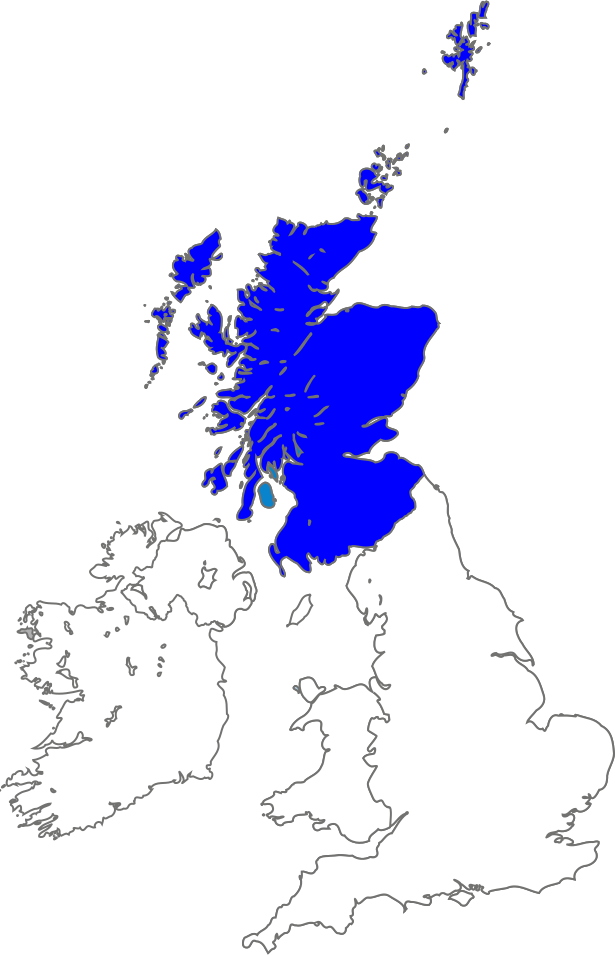
\includegraphics[height=0.5\textheight]{pix/map-scotland-blue.png}
\end{center}

\tiny{ Licensed under CC BY-SA 3.0 via Wikipedia -
\url{https://en.wikipedia.org/wiki/File:Map_of_Scotland_within_the_United_Kingdom.svg}
}


\end{frame}


% -----------------------------

\begin{frame}
\frametitle{Scottish Devolution}

\begin{itemize*}

\item \hl{1995} The \textit{Scottish Constitutional Convention}
(consisting of political parties, excluding Conservatives and SNP)
proposes a form of MMPR called the Additional Member System for the
new parliament.

\item \hl{1997}: UK Labour government holds referendum on creating a
Scottish Parliament. It passes with 74.3\% of the vote.


\end{itemize*}

\end{frame}

% https://en.wikipedia.org/wiki/Scottish_Constitutional_Convention
% http://www.gov.scot/Publications/2013/11/9348/16

% Devolved Decision Making, p. 8
% Wikipedia, Scottish Devolution Referendum, 1997


% -----------------------------

\begin{frame}
\frametitle{Municipal Reform}

\begin{itemize*}

\item \hl{2003}: Labour forms a coalition with Liberal Democrats. As a
condition, LibDems demand PR for municipal elections.

\item \hl{2004}: \textit{Local Governance (Scotland) Act} act is
passed, which legislates STV.

\item \hl{2007}: First STV elections.

\end{itemize*}

\end{frame}

% -----------------------------

\begin{frame}
\frametitle{How Scotland Won PR}

\begin{itemize*}

\item Long devolution campaign and adoption of PR for new parliament
(not switching from FPTP).

\item Coalition in which junior partner demands PR in exchange for
cooperation.

\end{itemize*}

\end{frame}

% ----------------------------
\begin{frame}

\bigtext{New Zealand}

\end{frame}

% ----------------------------
\begin{frame}
\frametitle{New Zealand}

New Zealand switched from FPTP to a MMPR system
in 1993. How did they do it?


\begin{center}
\includegraphics[height=0.5\textheight]{pix/map-new-zealand-blue.png}
\end{center}

\tiny{ Licensed under CC BY-SA 3.0 via Wikipedia -
\url{https://en.wikipedia.org/wiki/File:New_Zealand_location_map.svg}
}


\end{frame}

% -----------------------------

\begin{frame}
\frametitle{Background}

New Zealand holds national elections every three years.  Main
Parties:

\begin{small}
\begin{itemize*}

\item Labour: large centre-left party.

\item National: large centre-right party.

\item New Zealand First: centrist anti-immigration party. 

\item United Future: leftish party formed from the ashes of the United
party and Future New Zealand (2002 on)

\item Green: environmentalism.

\item Maori: Indigenous rights.

\item ACT: classical-liberal right-wing party.

\end{itemize*}
\end{small}


\end{frame}
% -----------------------------

\begin{frame}[plain]


\fullpich{pix/New_Zealand_1978.png}
{Tallies from Wikipedia: 
\url{https://en.wikipedia.org/wiki/New_Zealand_general_election,_1978}
}

\end{frame}


% -----------------------------

\begin{frame}[plain]


\fullpich{pix/New_Zealand_1981.png}
{Tallies from Wikipedia: 
\url{https://en.wikipedia.org/wiki/New_Zealand_general_election,_1981}
}

\end{frame}


% -----------------------------
\begin{frame}
\frametitle{Timeline}
\begin{itemize*}

\item \hl{1978,1981}: Wrong-way winners.

\item \hl{1985}: The Labour government implements a \textit{Royal Commission
on the Electoral System}, which recommends MMPR. 

\item \hl{1987}: Labour promises a referendum on MMPR but doesn't
implement it.

\item \hl{1990}: Labour (accidentally?) promises a referendum.
National promises a (non-binding) referendum. 

\end{itemize*}

% Source: from FPP to MMP (Wayback machine)
% http://www.elections.org.nz/voting/mmp/history-mmp.html

\end{frame}
% -----------------

\begin{frame}
\frametitle{Referendums}


Voters were asked whether to change the electoral
system and what alternative to choose. 

If voters chose to change the system, there would be a second
referendum the following year.


\end{frame}

% THESE SHOULD BE GRAPHS


% -----------------------------

% Source: http://www.elections.org.nz/voting/mmp/history-mmp.html
\begin{frame}
\frametitle{1992 Referendum Question, Part A}

\begin{block}{}
\begin{center}
Part A: Choose one Proposal
\begin{tabular}[c]{l|r}
\hline
 & \\
Retain FPP &  \\
\small{I vote to retain the present}  & 15.28\%\\
\small{First Past the Post System}  & \\
\hline
 & \\
Change System &  \\
\small{I vote for a change to}  & \textbf{81.72\%} \\
\small{the electoral system}  & \\
\hline
\end{tabular}
\end{center}
\end{block}

% Source: Wikipedia

\end{frame}


% -----------------------------

\begin{frame}
\frametitle{1992 Referendum Question, Part B}

\begin{block}{}
\begin{center}
Part B: Choose one Option
\begin{tabular}[c]{l|r}
\hline
 & \\
Preferential Voting (aka IRV) & 6.04\% \\
\hline
 & \\
Mixed-Member Proportional & \textbf{64.95\%} \\
\hline
 & \\
Supplementary Member & 5.12\% \\
\hline
 & \\
Single Transferable Vote & 16.00\% \\
\hline
 & \\
(Invalid) & 7.89\% \\
\hline
\end{tabular}
\end{center}
\end{block}


% Source: Wikipedia

\end{frame}



% -----------------------------

\begin{frame}
\frametitle{1992 Referendum Comments}

\begin{itemize*}

\item Having two questions meant voters could indicate that 
support for eliminating FPTP was much stronger than any consensus on
the replacement. 

\item The New Zealand government sent out information to all
households about the different voting systems for Part B. 

\item There was a 50\% double threshold (50\% + 1 vote, 50\% ridings)

\end{itemize*}

\end{frame}

% -----------------------------

\begin{frame}
\frametitle{1993 Referendum Question}


\begin{block}{}
\begin{center}
Choose one Proposal
\begin{tabular}[c]{l|r}
\hline
 & \\
First Past the Post (FPP) &  \\
\small{I vote to retain the present}  & 46.14\%\\
\small{First Past the Post System}  & \\
\small{as provided by the Electoral Act 1956}  & \\
\hline
 & \\
Mixed Member Proportional (MMP)  &  \\
\small{I vote for the proposed Mixed}  & \textbf{53.86\%} \\
\small{Member Proportional system as}  & \\
\small{provided by the Electoral Act 1993}  & \\
\hline
\end{tabular}
\end{center}
\end{block}

% Source: Wikipedia

\end{frame}




% ----------------------------
\begin{frame}
\frametitle{First MMPR elections}

\begin{itemize*}

\item \hl{1996}: National gets a plurality, and unexpectedly 
partners with New Zealand First (who campaigned against them!)

\item \hl{1999}: Labour wins 38.7\% of the vote, forms government with 
Alliance and Greens. 

\item \hl{2002}: Labour wins 41.2\% of the vote, forms government with 
United Future. Main issue: fight with Greens over GMOs.

\item \hl{2005}: Labour wins (41.1\%), forms coalition with
Progressive, with \textbf{supply and confidence} from NZ First, United 
Future.

\end{itemize*}
\end{frame}



% -----------------------------

\begin{frame}[plain]


\fullpich{pix/New_Zealand_1996.png}
{Tallies from Wikipedia: 
\url{https://en.wikipedia.org/wiki/New_Zealand_general_election,_1996}
}

\end{frame}


% -----------------------------

\begin{frame}[plain]


\fullpich{pix/New_Zealand_1999.png}
{Tallies from Wikipedia: 
\url{https://en.wikipedia.org/wiki/New_Zealand_general_election,_1999}
}

\end{frame}


% -----------------------------

\begin{frame}[plain]


\fullpich{pix/New_Zealand_2002.png}
{Tallies from Wikipedia: 
\url{https://en.wikipedia.org/wiki/New_Zealand_general_election,_2002}
}

\end{frame}


% -----------------------------

\begin{frame}[plain]


\fullpich{pix/New_Zealand_2005.png}
{Tallies from Wikipedia: 
\url{https://en.wikipedia.org/wiki/New_Zealand_general_election,_2005}
}

\end{frame}


% ----------------------------
\begin{frame}
\frametitle{More elections}

\begin{itemize*}

\item \hl{2008}: National wins 44.9\% of the vote, governs as minority
with supply and confidence from ACT, United Future, Maori parties.
National promises to ``reevaluate'' MMPR via referendum. 


\end{itemize*}

% Lots of drama in 2008 election. Find ads?

\end{frame}

% -----------------------------

\begin{frame}
\frametitle{Reform, Revisited}

\begin{itemize*}

\item \hl{2008}: National promises a referendum to revisit (and
possibly abolish) MMPR.

\item \hl{2011}: Referendum! Voters choose to keep MMPR with 57.7\% of
the (valid) vote. 

\item \hl{2012}: MMPR is reviewed and some amendments are made to
prevent tiny parties from getting extra list seats.

\end{itemize*}

% file:///home/pnijjar/pr-talk/bg-research/new-zealand/Electoral%20reform%20in%20New%20Zealand%20-%20Wikipedia,%20the%20free%20encyclopedia.html

\end{frame}

% -----------------------------

\begin{frame}
\frametitle{2011 Referendum Question, Part A}

\begin{block}{}
\begin{center}
Should New Zealand Keep the Mixed Member Proportional voting system?
\begin{tabular}[c]{l|r}
\hline
 & \\
Yes - keep MMP &  \\
\small{I vote to keep the MMP System}  & \textbf{56.17\%}\\
\hline
 & \\
No - change system &  \\
\small{I vote to change to}  & 41.06\% \\
\small{another system}  & \\
\hline
(Invalid) & 2.77\% \\
\hline
\end{tabular}
\end{center}
\end{block}

% Source: Wikipedia

\end{frame}


% -----------------------------

\begin{frame}
\frametitle{2011 Referendum Question, Part B}

\begin{block}{}
\begin{center}
\begin{small}
If New Zealand were to change to another voting system, which 
voting system would you choose?
\end{small}
\begin{tabular}[c]{l|r}
\hline
 & \\
First Past the Post  & 31.19\% \\
\hline
 & \\
Preferential Voting (aka IRV) & 8.34\% \\
\hline
 & \\
Single Transferable Vote & 11.19\% \\
\hline
 & \\
Supplementary Member & 16.14\% \\
\hline
 & \\
(Invalid) & \textbf{33.14\%} \\
\hline
\end{tabular}
\end{center}
\end{block}


% Source: Wikipedia

\end{frame}

% -----------------------------

\begin{frame}
\frametitle{2011 Referendum Comments}
\begin{itemize*}

\item The number of invalid ballots for Part B was enormous.

\item Support for MMP appears to have grown since the 1993 election.

\item Support for FPTP is still significant: over 30\%?

\end{itemize*}

\end{frame}


% ----------------------------
\begin{frame}
\frametitle{Recent Elections}

\begin{itemize*}
\item \hl {2011}: National wins 47.3\% of the vote, governs as
minority with supply and confidence from ACT, United Future, Maori.

\item \hl {2014}: National wins 47.0\% of the vote, 60/121 seats,
governs as minority with supply and confidence from ACT, United
Future, Maori.

\end{itemize*}
\end{frame}

% -----------------------------

\begin{frame}[plain]


\fullpich{pix/New_Zealand_2011.png}
{Tallies from Wikipedia: 
\url{https://en.wikipedia.org/wiki/New_Zealand_general_election,_2011}
}

\end{frame}


% -----------------------------

\begin{frame}[plain]


\fullpich{pix/New_Zealand_2014.png}
{Tallies from Wikipedia: 
\url{https://en.wikipedia.org/wiki/New_Zealand_general_election,_2014}
}

\end{frame}


% -----------------------------

\begin{frame}
\frametitle{How New Zealand Won PR}

\begin{itemize*}

\item Two wrong-way winners that made Labour (and NZ voters) mad.

\item Government report followed by foot-dragging, followed by
election promises.

\item Two successful referendums.

\item Wacky coalitions, then three Labour victories in a row, followed by
promises to re-evaluate the system.

\item Another referendum which supports MMPR.

\item The system is improved.


\end{itemize*}

\end{frame}



% ----------------------------
\begin{frame}

\bigspookytext{The Canadian story}

\end{frame}


% ----------------------------
\begin{frame}
\frametitle{Trivia Interlude}

\begin{center}
\begin{large}
\hl{What has the closest Canada has come to winning
proportional representation at any level of government?}
\end{large}
\end{center}

\end{frame}


% -----------------------------

\begin{frame}
\frametitle{Surprise!}

\begin{itemize*}

\item \hl{1920}: Manitoba Liberal party introduces STV for Winnipeg seats
(and IRV for rural seats in 1924).

\item \hl{1924}: Alberta Progressive party introduces STV for Calgary and
Edmonton (and IRV everywhere else).

\item \hl{1916-1928}: 18 municipalities introduce STV for municipal
elections.

\end{itemize*}

\end{frame}

% Source: Electoral Reform in Canada, Louis Massicotte, p. 113
% Source: AV in Canada: On Power and Politics

% -----------------------------

\begin{frame}
\frametitle{No Surprise!}

\begin{itemize*}

\item \hl{1959} Alberta Social Credit party institutes FPTP
everywhere.

\item \hl{1956} Manitoba redistributes ridings and eliminates STV.

\end{itemize*}

\pause

Official reasons: STV and IRV are too difficult to tally, Winnipeg was
underrepresented...

Unofficial reasons: Hmmmm...

(Also see: British Columbia 1951-1953)

\end{frame}

% https://en.wikipedia.org/wiki/Manitoba_general_election,_1953
% https://en.wikipedia.org/wiki/Manitoba_general_election,_1958


% ----------------------------
\begin{frame}

\bigtext{British Columbia}

\end{frame}



% -----------------------------

\begin{frame}[plain]


\fullpich{pix/British_Columbia_Provincial_Election_1996.png}
{Tallies from Wikipedia: 
\url{https://en.wikipedia.org/wiki/British_Columbia_general_election,_1996}
}

\end{frame}


% -----------------------------

\begin{frame}[plain]


\fullpich{pix/British_Columbia_Provincial_Election_2001.png}
{Tallies from Wikipedia: 
\url{https://en.wikipedia.org/wiki/British_Columbia_general_election,_2001}
}

\end{frame}


% -----------------------------

\begin{frame}
\frametitle{British Columbia Timeline}

\begin{itemize*}

\item \hl{1996}: Wrong-way winner. Liberals lose.

\item \hl{2001}: Liberals under Gordon Campbell get lopsided majority,
promise electoral reform.

\item \hl{2002}: Gordon Gibson of Fraser Institute recommends a
\textbf{citizens assembly} and referendum.

\item \hl{March 2004}: \textit{Electoral Reform Referendum Act}
demands 60\% supermajority.

\item \hl{Dec 2004}: Citizens Assembly recommends STV.

\end{itemize*}

\end{frame}

% Carty, Blais, Fornier: When Citizens Choose to Reform SMP, p. 145
% https://en.wikipedia.org/wiki/Citizens%27_Assembly_on_Electoral_Reform_%28British_Columbia%29



% -----------------------------

\begin{frame}
\frametitle{2005 BC Referendum}

\begin{block}{}
\begin{center}
Should British Columbia change to the BC-STV electoral system, as
recommended by the Citizens' Assembly on Electoral Reform?
\begin{tabular}[c]{l|r|r}
Option & \% Vote & Num Ridings \\
\hline
 & & \\
Yes &  \textbf{57.7\%} & 77\\
\hline
 & & \\
No &   43.3 & 2 \\
\hline
\end{tabular}
\end{center}
\end{block}


\end{frame}

% Source: Wikipedia
% Chief electoral officer report, p. 42 

% -----------------------------

\begin{frame}
\frametitle{Referendum}

\begin{itemize*}


\item Campbell and the Liberals  ``officially neutral''. The NDP was
split (despite having endorsed PR officially). The Green leader
Adrienne Carr made statements opposing STV (!)

\item Second referendum was promised for 2009, with new electoral
boundaries filled in, and funding offered to pro- and anti- groups.

\end{itemize*}

\end{frame}


% -----------------------------

\begin{frame}
\frametitle{2009 BC Referendum Question}

\begin{block}{}
\begin{center}
\begin{small}
Which electoral system should British Columbia use to elect members to
the provincial Legislative Assembly?
\end{small}
\begin{tabular}[c]{l|r|r}
Option & \% Vote & Ridings \\
\hline
 & & \\
\small{The existing electoral system} &  &\\
\small{(First-Past-the-Post)} &  \textbf{60.9\%} & 77 \\
\hline
 & & \\
\small{The single transferable vote} &   & \\
\small{electoral system (BC-STV)} &   39.1\% & 8 \\
\small{proposed by the Citizens'} &   &  \\
\small{Assembly on Electoral Reform?} &   &  \\
\hline
\end{tabular}
\end{center}
\end{block}


\end{frame}

% Source: Wikipedia
% Chief electoral officer report, p. 42 

% -----------------------------

\begin{frame}
\frametitle{Summary}


\begin{block}{}
\begin{center}
\begin{tabular}[c]{l|r|r}
Initiative & Change System & No Change \\
\hline
BC 2005 & 57.7 & 42.3 \\
PEI 2005 & 36.4 & 63.6 \\
ON 2007 & 36.9 & 63.1 \\
BC 2009 & 39.1 & 60.9 \\
\hline
\end{tabular}
\end{center}
\end{block}

Also, attempts in Quebec (ended 2007) and New Brunswick (ended 2006).

Each of these losses hurt the movement. The BC 2009 loss was
crippling.



\end{frame}


% -----------------------------

\begin{frame}
\frametitle{From Conservative Platform}

\textit{
The Liberals and NDP would make these democratic changes to our
democratic system and impose them on Canadians without consultation
because when Canadians are asked -- as they have been in
Ontario, British Columbia, and Prince Edward Island -- they've
\textbf{chosen the status quo}. 
}

\small{(emphasis mine)}

\end{frame}


% ----------------------------
\begin{frame}

\bigspookytext{Lessons}

\end{frame}



% -----------------------------

\begin{frame}
\frametitle{Lesson: Wacky Elections}

Lopsided results and wrong-way majorities motivate electoral reform.
(NZ, BC, Lesotho)

Phony majorities and vote-splitting is ``business as usual.''

\end{frame}

% -----------------------------

\begin{frame}
\frametitle{Lesson: Inertia}

Moving from FPTP to anything else is really hard.

Once electoral reform has started it can keep going:
\begin{itemize*}

\item Voting system improvements (NZ, Lesotho)

\item Reversions to FPTP (Canada)

\end{itemize*}

Rejected electoral reform attempts cause setbacks.

\end{frame}

% -----------------------------

\begin{frame}
\frametitle{Lesson: FPTP Corrupts}

Governments that win majorities under FPTP have little incentive to
change the system unless they get ripped off or can be held
accountable.

Governments can sabotage electoral reform:
\begin{small}
\begin{itemize*}

\item ``Official'' neutrality.

\item Supermajority requirements.

\item Dragging feet until it is too late.

\end{itemize*}
\end{small}

\end{frame}


% -----------------------------

\begin{frame}
\frametitle{Lesson: Rocky Beginnings}

Expect the first few elections under PR to be rocky. 

People will be grumpy with weird outcomes.

Politics will still be dirty.

\end{frame}


% -----------------------------

\begin{frame}
\frametitle{Lesson: Life Under PR}

Democracy means parties you don't like will win power.

PR can make it harder to ``kick the rascals out''.

Coalition agreements add post-election drama and can be unexpected (NZ
1996). 

FPTP defenders make some arguments that are worth considering (and
others that are ridiculous). 

\end{frame}


% -----------------------------

\begin{frame}
\frametitle{Lesson: Referendums}

New Zealand has demonstrated that clear multi-part referendums can
work well.

The New Zealand referenda clearly distinguished between evaluating
FPTP and choosing a different system.

\end{frame}


% ----------------------------
\begin{frame}

\bigspookytext{What comes next?}

\end{frame}


% ----------------------------
\begin{frame}
\frametitle{Municipal Ranked Ballots}

The Ontario government will allow (not force) municipalities to use ranked ballots for elections.

``Ranked ballots'' are not a voting system, but can be used to
implement voting systems: 

\begin{itemize*}

\item Proportional: Single-Transferable Vote (STV)

\item Non-proportional: Instant Runoff/Alternative Vote 
(IRV or AV), Borda Counts... 

\end{itemize*}
\end{frame}

% ---------------------------------
\begin{frame}
\frametitle{What to do?}

Should we advocate the use of ranked ballots in the region of
Waterloo? For mayors? City councillors? Regional councillors? 

Should we reject ranked ballots if they will not be used to 
implement proportional systems?

What happens if we reject electoral change again?

\end{frame}


% ----------------------------
\begin{frame}
\frametitle{Federal Liberal Promises}


From: Liberal platform document \textit{Real Change: A Plan for a New Middle Class}, p. 28


\textbf{We will make every vote count.}

\textit{
We are committed to ensuring that 2015 will be the last federal
election conducted under the first-past-the-post voting system.
}

\end{frame}



% ----------------------------
\begin{frame}

\textit{
We will convene an all-party Parliamentary committee to review a wide
variety of reforms, such as ranked ballots, proportional
representation, mandatory voting, and online voting.
}

\textit{
This committee will deliver its recommendations to Parliament. Within
18 months of forming government, we will introduce legislation to
enact electoral reform.
}


\end{frame}



% ----------------------------
\begin{frame}
\frametitle{Uh oh}

The Liberals are \textit{not} promising to implement proportional representation. 

They are promising a multi-party committee which can recommend
whatever it wants. 


\end{frame}


% ----------------------------
\begin{frame}
\frametitle{More uh oh}

\begin{itemize*}

\item Electoral catastrophe? No.

\item Trudeau supports PR? Not during his leadership campaign.

\item Liberals benefit from PR? Not necessarily. 
IRV is better for big-tent centrist parties.

\item Liberals ripped off by FPTP? Not more than usual.

\item Government won phony majority? Yes.

\item Official opposition advocating for PR? No.

\end{itemize*}


\end{frame}


% ----------------------------
\begin{frame}
\frametitle{What can we do?}

We cannot \textit{force} the Liberals to adopt PR.
But maybe we can...

\begin{small}
\begin{itemize*}

\item Keep pressure on all parties in parliament.

\pause

\item Criticize attempts by the government to sabotage the process.

\pause

\item Broaden support and awareness of electoral reform.

\pause

\item Take advantage of municipal electoral reform.

\pause

\item Keep proportional representation multipartisan.

\pause

\item Stop fighting among ourselves!

\end{itemize*}
\end{small}

\end{frame}

% -----------------------------

\begin{frame}[plain]
\bigtext{How? (You already know how)}

\end{frame}


% -----------------------------

\begin{frame}
\frametitle{Learn}

Can you explain FPTP and PR to others?

Are you comfortable with the tradeoffs yourself?

What things do you want from democracy?

\end{frame}


% -----------------------------

\begin{frame}
\frametitle{Get Involved}

Fair Vote Canada is holding a meeting on: Monday Nov 9, 7pm, Heuther Hotel: Working with MPs.

You can join the leadnow.ca campaign.

You can make other local activities (discussions, learning circles,
public events) happen as well.

\end{frame}


% -----------------------------

\begin{frame}[plain]


\fullpich{pix/sharon-fvc-booth.jpg}
{Fair Vote Canada, CC-BY 
\url{http://www.fairvotewrc.ca/election-simulation-at-kultrun/}
}

\end{frame}


% -----------------------------

\begin{frame}
\frametitle{Keep Up the Pressure}

Let your MP know you are vigilant.

In-person meetings are most effective,
followed by snail mail, email, and then signing petitions.

\end{frame}


% -----------------------------

\begin{frame}
\frametitle{Positive signs}

Awareness of the term ``First-Past-the-Post'' is rising.

Some big players (eg leadnow.ca) are taking up this cause.

The kids are all right.

The Conservatives mentioned electoral reform in their platform.

\end{frame}

% ----------------------------
\begin{frame}

\bigspookytext{The End}

\end{frame}

% ----------------------------
\begin{frame}

\bigspookytext{Feedback}

\end{frame}


% -----------------------------

\begin{frame}
\frametitle{Thank You!}

To all of you for attending.

To those who offered publicity help.

To everybody who put up with me obsessing about this talk for a month
and a half.

To people who helped with setup and takedown.

To The Working Centre for hosting the space.

\end{frame}



% ----------------------------
\begin{frame}

\bigspookytext{Questions? Clarifications? Pitchforks?}

\end{frame}

% -----------------------------

\begin{frame}
\frametitle{License}

This slideshow is released under a Creative Commons Attribution
Sharealike 4.0 license. 

If the screenshots I grabbed are not eligible for CC-BY-SA licensing,
then they should be omitted from derivative works. 

\end{frame}



% ----------------------------
\begin{frame}

\bigspookytext{References}

\end{frame}


% -----------------------------

\begin{frame}[c,allowframebreaks]
\frametitle{References: FPTP}

\printbibliography[keyword=fptp,notkeyword=tallies]

\end{frame}


% -----------------------------

\begin{frame}[c,allowframebreaks]
\frametitle{References: Lesotho}


\printbibliography[keyword=lesotho,notkeyword=tallies]


\end{frame}


% -----------------------------

\begin{frame}[c,allowframebreaks]
\frametitle{References: Scotland}


\printbibliography[keyword=scotland,notkeyword=tallies]


\end{frame}

% -----------------------------

\begin{frame}[c,allowframebreaks]
\frametitle{References: New Zealand}


\printbibliography[keyword=new-zealand,notkeyword=tallies]


\end{frame}



% -----------------------------

\begin{frame}[c,allowframebreaks]
\frametitle{References: British Columbia}


\printbibliography[keyword=british-columbia,notkeyword=tallies]


\end{frame}

% -----------------------------

\begin{frame}[c,allowframebreaks]
\frametitle{References: (Rest of) Canada}


\printbibliography[keyword=canada,notkeyword=tallies]


\end{frame}

% -----------------------------

\begin{frame}[c,allowframebreaks]
\frametitle{References: Election Tallies}


\printbibliography[keyword=tallies]


\end{frame}




% ----------------------------
\begin{frame}

\bigspookytext{Extra Slides}

\end{frame}


% -----------------------------

\begin{frame}

\bigtext{Other Provinces}

\end{frame}


% -----------------------------

\begin{frame}
\frametitle{2005: Prince Edward Island}

\begin{itemize*}

\item \hl{2003}: Government appoints one-person commission (Norman H
Carruthers) to conduct consultations and study electoral reform.

\item \hl{2005}: PEI holds plebicite on MMPR
system (with usual supermajority).

\item 36.4\% vote in
favour, passing in 2/27 ridings.

\end{itemize*}

\end{frame}


% -----------------------------

\begin{frame}
\frametitle{PEI Comments}

\begin{itemize*}

\item Referendum was not held during an election. It had fewer polling
stations. Turnout was low.

\item Neither the Liberals nor Conservatives supported the change.

\end{itemize*}

\end{frame}



% -----------------------------

\begin{frame}
\frametitle{2006: New Brunswick}

\begin{itemize*}

\item \hl{2003}: Commission on Legislative Democracy established by
Conservative Bernard Lord. 

\item \hl{2005}: Commission recommends MMPR system and referendum.

\item \hl{2006}: Conservatives lose election (in wrong-way winner!),
and Liberals drop the recommendation.

\end{itemize*}

\end{frame}

% -----------------------------

\begin{frame}
\frametitle{Quebec}

\begin{itemize*}

\item \hl{2003}: Estates General on Reform of Democratic Commissions
recommends regional MMPR.

\item \hl{2004}: Draft bill proposed to Quebec assembly. 

\item \hl{2006}: Appointed Citizens Committee rejects bill as written,
but recommends a different form of MMPR. 

\item \hl{2007}: Chief Electoral Officer releases report recommending
a switch. 

\item And then...?

\end{itemize*}

% http://www.electionsquebec.qc.ca/english/provincial/media/reform-of-the-voting-system.php

\end{frame}

% -----------------------------

\begin{frame}
\frametitle{2007: Ontario}

\begin{itemize*}

\item \hl{2004}: Liberals announce Citizens' Assembly and referendum

\item \hl{2007}: Citizens' Assembly recommends MMPR. 

\item \hl{2007}: Ontario holds referendum with usual supermajority
thresholds. 

\item 36.9\% vote for MMPR, passing in 5/107 ridings.


\end{itemize*}
\end{frame}

% ----------------------------
\begin{frame}
\frametitle{Ontario Comments}

\begin{itemize*}

\item Liberals: Officially neutral. PC: against. NDP: supposedly
in favour. 

\item Media coverage was overwhelmingly negative. 

\item Government education campaign: terrible.

\end{itemize*}

\end{frame}



% ----------------------------
\begin{frame}

\bigtext{Canada}

\end{frame}



% -----------------------------

\begin{frame}
\frametitle{2004: Law Commission of Canada}

\begin{itemize*}

\item \hl{2004}: Law Commission of Canada drafts a report recommending
MMPR.

\item \hl{2005}: NDP forces Liberals to establish a Committee to
review electoral reform. They reject a Citizens Assembly process.
They set up procedures to report by Feb 2006.

% Massicotte: p. 122

\item \hl{2006}: Liberal government falls and is replaced by
Conservatives. 

\item And then...?

\end{itemize*}

\end{frame}

% ----------------------------
\begin{frame}
\frametitle{2008-2012: Charter Challenge}

The Association for the Advancement of Democratic
Rights took the Quebec government to court over FPTP, citing Charter:

\begin{small}
\begin{itemize*}

\item Section 3: All citizens have the right to vote, but not all
votes are counted. 

\item Section 15: FPTP discriminates against women, minorities, and
supporters of fringe parties.

\end{itemize*}
\end{small}

In 2009 a Quebec judge ruled against the case. In 2012 their appeal to
the Supreme Court was dismissed.

\end{frame}

% -----------------------------

\begin{frame}
\frametitle{Sidenote: IRV in BC}

\hl{1951}: British Columbia introduces (non-proportional) IRV to keep
the CCF from benefiting from vote splitting.

\hl{1953}: British Columbia Social Credit party abolishes IRV in
favour of FPTP.

\end{frame}


% -----------------------------

\begin{frame}
\frametitle{What do you want from democracy?}

\begin{itemize*}

\item To help elect people you like?

\item To prevent people you dislike from getting power?

\item To give governments strong mandates?

\item To have strong local representation?

\item To introduce new ideas and innovation?

\item To let governments make unpopular but necessary decisions?

\item To kick the rascals out?

\end{itemize*}

\end{frame}

% -----------------------------


\begin{frame}
\frametitle{Dec 3 2014 vote}

\textit{
That, in the opinion of the House: (a) the next federal election
should be the last conducted under the current first-past-the-post
electoral system which has repeatedly delivered a majority of seats to
parties supported by a minority of voters, or under any other
winner-take-all electoral system; and (b) a form of mixed-member
proportional representation would be the best electoral system for
Canada.
}


\end{frame}

% ref: fairvote Vote 291 details
% -----------------------------


\begin{frame}[plain]


\fullpicv{pix/2014-12-03-vote-fvc.png}
{ Source: Fair Vote Canada (via Facebook) }

\end{frame}


% -----------------------------
\begin{frame}
\frametitle{No MMP}

\fullpicv{pix/nommp-01.png}
{Source: 2007 NO MMP Campaign}
\end{frame}

% -----------------------------

\begin{frame}
\frametitle{No MMP - back}

\fullpicv{pix/nommp-02.png}
{Source: 2007 NO MMP Campaign}


\end{frame}

\end{document}
